\documentclass[landscape,a0paper,fontscale=0.4]{baposter}
% make fontscale bigger to get smaller fonts

\tracingstats=2

\usepackage{times}
\usepackage{calc}
\usepackage{url}
\usepackage{graphicx}
\usepackage{amsmath}
\usepackage{amssymb}
\usepackage{relsize}
\usepackage{multirow}
\usepackage{caption}
% \usepackage[authoryear,round]{natbib}
\usepackage[hidelinks]{hyperref}
\usepackage{booktabs}

\usepackage{graphicx}
\usepackage{multicol}
\usepackage[T1]{fontenc}
\usepackage{ae}

\usepackage{minted}
\setminted{fontsize=\scriptsize}

\graphicspath{{images/}}

 %%%%%%%%%%%%%%%%%%%%%%%%%%%%%%%%%%%%%%%%%%%%%%%%%%%%%%%%%%%%%%%%%%%%%%%%%%%%%%%%
 %%%% Some math symbols used in the text
 %%%%%%%%%%%%%%%%%%%%%%%%%%%%%%%%%%%%%%%%%%%%%%%%%%%%%%%%%%%%%%%%%%%%%%%%%%%%%%%%
 % Format 
\newcommand{\R}{\mathbb{R}}
\newcommand{\E}{\mathbb{E}}
\renewcommand{\P}{\mathbb{P}}
\newcommand{\st}{\,\colon\,}
\newcommand{\bone}{\mathbf{1}}
\newcommand{\var}{\mathop{\mbox{Var}}}
\newcommand{\cov}{\mathop{\mbox{cov}}}
\newcommand{\tskit}{{\texttt{tskit}}}
\newcommand{\branch}{\mbox{Branch}} % branch stat
\newcommand{\branchp}{\mbox{Branch}_+} % polarised
\newcommand{\site}{\mbox{Site}} % site stat
\newcommand{\sitep}{\mbox{Site}_+} % polarised
\newcommand{\node}{\mbox{Node}} % node stat
\newcommand{\nodep}{\mbox{Node}_+} % polarised
\newcommand{\given}{\;\vert\;}


 %%%%%%%%%%%%%%%%%%%%%%%%%%%%%%%%%%%%%%%%%%%%%%%%%%%%%%%%%%%%%%%%%%%%%%%%%%%%%%%%
 % Multicol Settings
 %%%%%%%%%%%%%%%%%%%%%%%%%%%%%%%%%%%%%%%%%%%%%%%%%%%%%%%%%%%%%%%%%%%%%%%%%%%%%%%%
 \setlength{\columnsep}{0.7em}
 \setlength{\columnseprule}{0mm}


 %%%%%%%%%%%%%%%%%%%%%%%%%%%%%%%%%%%%%%%%%%%%%%%%%%%%%%%%%%%%%%%%%%%%%%%%%%%%%%%%
 % Save space in lists. Use this after the opening of the list
 %%%%%%%%%%%%%%%%%%%%%%%%%%%%%%%%%%%%%%%%%%%%%%%%%%%%%%%%%%%%%%%%%%%%%%%%%%%%%%%%
 \newcommand{\compresslist}{%
 \setlength{\itemsep}{1pt}%
 \setlength{\parskip}{0pt}%
 \setlength{\parsep}{0pt}%
 }

%%%%%%%%%%%%%%%%%%%%%%%%%%%%%%%%%%%%%%%%%%%%%%%%%%%%%%%%%%%%%%%%%%%%%%%%%%%%%%
%%% Other Macros
%%%%%%%%%%%%%%%%%%%%%%%%%%%%%%%%%%%%%%%%%%%%%%%%%%%%%%%%%%%%%%%%%%%%%%%%%%%%%%
% \renewcommand{\labelenumi}{\alph{enumi})}
% \renewcommand{\theenumi}{\alph{enumi})}
\newcommand{\postercaption}[1]{\begin{minipage}{\linewidth}\center\smaller
  {#1}\end{minipage}}



%%%%%%%%%%%%%%%%%%%%%%%%%%%%%%%%%%%%%%%%%%%%%%%%%%%%%%%%%%%%%%%%%%%%%%%%%%%%%
%% Begin of Document
%%%%%%%%%%%%%%%%%%%%%%%%%%%%%%%%%%%%%%%%%%%%%%%%%%%%%%%%%%%%%%%%%%%%%%%%%%%%%
\begin{document}

% Define some colors
\definecolor{tskitMint}{RGB}{93,199,148}  % 5dc794
\definecolor{tskitBlue}{RGB}{31,78,102}  % 1f4e66

\definecolor{silver}{cmyk}{0,0,0,0.3}
\definecolor{black}{cmyk}{0,0,0.0,1.0}
\definecolor{white}{cmyk}{0,0,0.0,0.0}
\definecolor{darkSilver}{cmyk}{0,0,0,0.1}

\definecolor{darkYellow}{cmyk}{0,0,1.0,0.5}
\definecolor{yellow}{cmyk}{0,0,0.9,0.0}
\definecolor{reddishyellow}{cmyk}{0,0.22,1.0,0.0}
\definecolor{lightyellow}{cmyk}{0,0,0.3,0.0}
\definecolor{lighteryellow}{cmyk}{0,0,0.1,0.0}
\definecolor{lightestyellow}{cmyk}{0,0,0.05,0.0}

\definecolor{darkCyan}{cmyk}{1,1,0,0.5}
\definecolor{cyan}{cmyk}{1,0,0,0.0}
\definecolor{lightcyan}{cmyk}{0.3,0,0,0.0}
\definecolor{lightercyan}{cmyk}{0.1,0,0,0.0}
\definecolor{lightestcyan}{cmyk}{0.05,0,0,0.0}

%%%%%%%%%%%%%%%%%%%%%%%%%%%%%%%%%%%%%%%%%%%%%%%%%%%%%%%%%%%%%%%%%%%%%%%%%%%%%
%% Here starts the poster
%%---------------------------------------------------------------------------
%% Format it to your taste with the options
%%%%%%%%%%%%%%%%%%%%%%%%%%%%%%%%%%%%%%%%%%%%%%%%%%%%%%%%%%%%%%%%%%%%%%%%%%%%%
\begin{poster}{
 % Show grid to help with alignment
 grid=false,
 % Column spacing
 colspacing=0.7em,
 % Color style
 headerColorOne=tskitMint,
 borderColor=tskitBlue,
 % Format of textbox
 textborder=faded,
 % Format of text header
 headerborder=open,
 headershape=roundedright,
 headershade=plain,
 background=none,
 bgColorOne=tskitMint,
 headerheight=0.12\textheight}
 % Eye Catcher
 { \includegraphics[height=0.12\textheight]{tskit_logo}
 }
 % Title
 {\Huge \tskit{}: \sc working with tree sequences}
 % Authors
  {\sf %Sans Serif
    Ben Jeffery${}^\ddagger$,
    Jerome Kelleher$^{\ddagger}$,
    Nathaniel Pope${}^\dagger$,
    Peter Ralph${}^\dagger$,
    \\  \vspace{-1.0mm}
    Georgia Tsambos,${}^{\dagger\S}$,
    Yan Wong$^{\ddagger}$,
    and the rest of the tskit-dev group.
    \\  \vspace{-1.0mm}
    Code: \url{github.com/petrelharp/progen-2023}. 
    \\  \vspace{-1.0mm}
    {\small \textit{$\dagger$ University of Oregon} } %\\ \vspace{-0.5em}
    {\small \textit{$\ddagger$ University of Oxford} } %\\ \vspace{-0.5em}
    {\small \textit{$\S$ University of Washington}} \\
  }
 % University logo
 {
  \begin{tabular}{r}
    \includegraphics[height=0.12\textheight]{oxford-logo.jpeg}
      \hspace{1em}
    \includegraphics[height=0.12\textheight]{UOSignature-STK-BLK}\\
  \end{tabular}
 }

%%%%%%%%%%%%%%%%%%%%%%%%%%%%%%%%%%%%%%%%%%%%%%%%%%%%%%%%%%%%%%%%%%%%%%%%%%%%%%
%%% Now define the boxes that make up the poster
%%%---------------------------------------------------------------------------
%%% Each box has a name and can be placed absolutely or relatively.
%%% The only inconvenience is that you can only specify a relative position 
%%% towards an already declared box. So if you have a box attached to the 
%%% bottom, one to the top and a third one which should be inbetween, you 
%%% have to specify the top and bottom boxes before you specify the middle 
%%% box.
%%%%%%%%%%%%%%%%%%%%%%%%%%%%%%%%%%%%%%%%%%%%%%%%%%%%%%%%%%%%%%%%%%%%%%%%%%%%%%

%%%%%%%%%%%%%%%%%%%%%%%%%%%%%%%%%%%%%%%%%%%%%%%%%%%%%%%%%%%%%%%%%%%%%%%%%%%%%%
\begin{posterbox}[name=inout,column=0,span=1]{Integrated metadata}
%%%%%%%%%%%%%%%%%%%%%%%%%%%%%%%%%%%%%%%%%%%%%%%%%%%%%%%%%%%%%%%%%%%%%%%%%%%%%%

    \tskit now has integrated metadata.
    For instance,
    the complete ARG for 1.26 million SARS-Cov-2 genomes: fits in 57MB!
    Loads in < 1s!

\begin{minted}{bash}
ls -lh SARS-Cov-2-ARG.ts.tsz
\end{minted}
{\scriptsize \verb|-rw-rw-r-- 1 jk jk 57M Mar  2 13:32 SARS-Cov-2-ARG.ts.tsz|}
\begin{minted}{python}
ts = tszip.decompress("SARS-Cov-2-ARG.ts.tsz")
\end{minted}
{\scriptsize
\begin{verbatim}
CPU times: user 775 ms, sys: 533 ms, total: 1.31 s
Wall time: 842 ms
\end{verbatim}
}
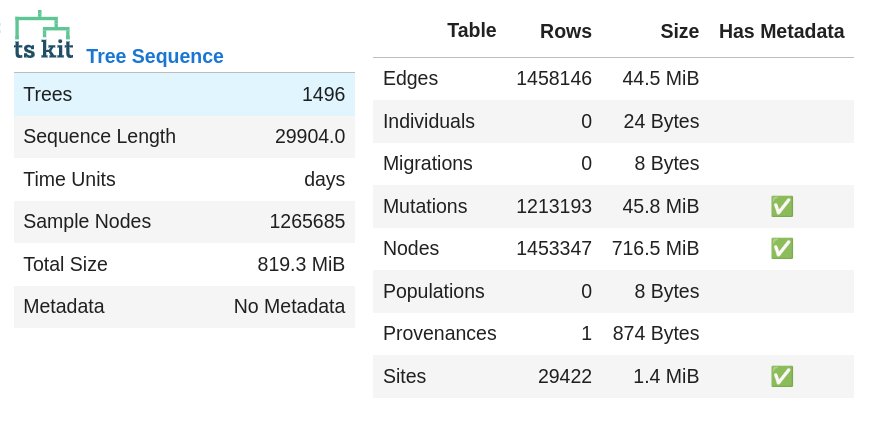
\includegraphics[width=0.5\textwidth]{sc2_ts.png}

\paragraph{Integrated data model} linking nodes, edges, sites and mutations and external metadata and debug information:

\begin{multicols}{2}
\begin{minted}{python}
ts.tables.sites[:5]
\end{minted}
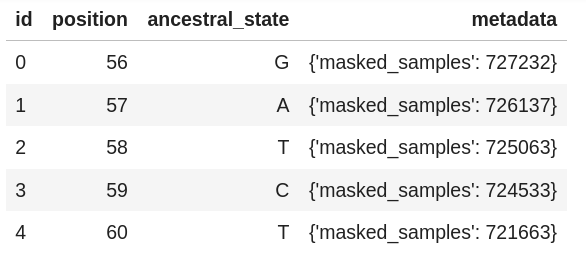
\includegraphics[width=0.5\textwidth]{sc2_sites}

\begin{minted}{python}
ts.tables.mutations[ts.mutations_site == 0]
\end{minted}
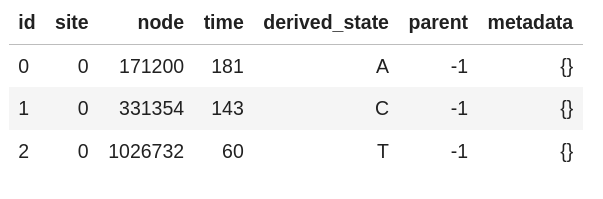
\includegraphics[width=0.5\textwidth]{sc2_muts}
\end{multicols}

\begin{minted}{python}
dataclasses.asdict(ts.node(1026732))
\end{minted}
\tiny
\begin{minted}{python}
{'id': 1026732,
 'flags': 1,
 'time': 60.0,
 'population': -1,
 'individual': -1,
 'metadata': {'Imputed_lineage': 'B.1.1.7',
  'Nextclade_pango': 'B.1.1.7',
  'clade': '20I (Alpha, V1)',
  'country': 'Germany',
  'date': '2021-05-01',
  'date_submitted': '2021-05-17',
  'gisaid_epi_isl': 'EPI_ISL_2122637',
  'host': 'Human',
  'sc2ts_qc': {'num_masked_sites': 150,
   'original_base_composition': {'-': 103,
    'A': 8902,
    'C': 5473,
    'G': 5847,
    'T': 9578},
   'original_md5': '8ca8e5ad1f098aa806126f2439810d7a'},
  'strain': 'Germany/un-RKI-I-137988/2021',
  'totalSubstitutions': 36.0}}
\end{minted}

\end{posterbox}
%%%%%%%%%%%%%%%%%%%%%%%%%%%%%%%%%%%%%%%%%%%%%%%%%%%%%%%%%%%%%%%%%%%%%%%%%%%%%%

%%%%%%%%%%%%%%%%%%%%%%%%%%%%%%%%%%%%%%%%%%%%%%%%%%%%%%%%%%%%%%%%%%%%%%%%%%%%%%
\begin{posterbox}[name=interop,column=0,row=0,span=1,below=inout]{Interfaces and interoperability}
%%%%%%%%%%%%%%%%%%%%%%%%%%%%%%%%%%%%%%%%%%%%%%%%%%%%%%%%%%%%%%%%%%%%%%%%%%%%%%

\begin{itemize} \compresslist
    \item Well-tested API used by many software packages: SLiM, fwdpy11, msprime, tsinfer/tsdate, Relate, etc.
    \item Available in multiple programming languages:
        \includegraphics[width=2em]{C_Logo}
        \includegraphics[width=2em]{python-logo-master-v3-TM-flattened}
        \includegraphics[width=2em]{RustLogo}
        
\includegraphics[width=2em]{R-logo}
    \item Runs in-browser (no install required!) for quick demos / teaching (see screenshot)
    \item Can represent full Ancestral Recombination Graphs; includes ARG likelihood calculations.
    \item Efficient processing of large genomic datasets (Covid ARG has ~1.3M samples, bigger ones coming)
    \item Interoperable with other packages (VCF output for sequence data, newick/nexus output e.g. to Dendropy, numpy arrays e.g. to scikit-allel)
\end{itemize}

% \begin{minted}{python}
% ts = msprime.sim_ancestry(2, sequence_length=600,
%         recombination_rate=1e-3, random_seed=7)
% ts = msprime.sim_mutations(ts, rate=2e-3, random_seed=9)
% 
% css = (".tree .plotbox {transform: skewY(0.7rad) "
%         "translateY(-50px)}")
% ts.draw_svg(size=(700, 200), x_scale="treewise",
%         style=css, mutation_labels={})
% \end{minted}

    \includegraphics[width=0.5\textwidth]{JupyterLite}

\end{posterbox}
%%%%%%%%%%%%%%%%%%%%%%%%%%%%%%%%%%%%%%%%%%%%%%%%%%%%%%%%%%%%%%%%%%%%%%%%%%%%%%

%%%%%%%%%%%%%%%%%%%%%%%%%%%%%%%%%%%%%%%%%%%%%%%%%%%%%%%%%%%%%%%%%%%%%%%%%%%%%%
\begin{posterbox}[name=overview,column=1,row=0,span=2]{Overview}
%%%%%%%%%%%%%%%%%%%%%%%%%%%%%%%%%%%%%%%%%%%%%%%%%%%%%%%%%%%%%%%%%%%%%%%%%%%%%%

    \begin{center}
        \huge
        ``\tskit{}: launching your genomes into the time dimension''
    \end{center}

- very brief intro/description statement
- what's on the website
- emphasize that (a) it does stuff fast and quick, and (b) it gives us a time dimension
    * tagline: "launching your genomes into the time dimension"?
- how to contribute
- bigger ecosystem: what else uses tskit?

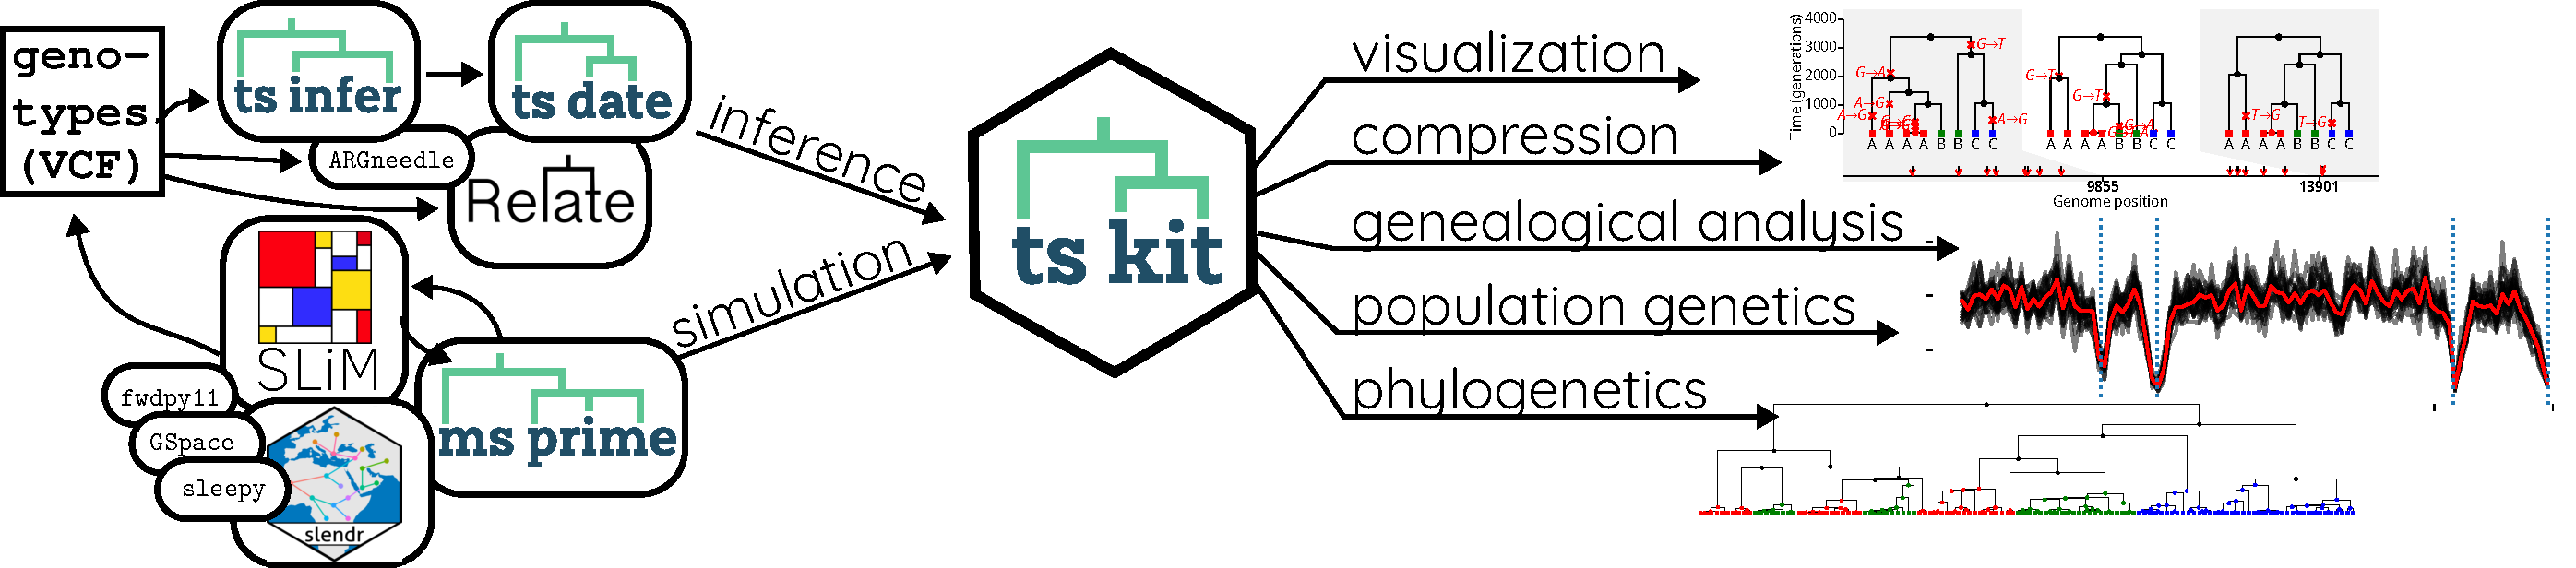
\includegraphics[width=\textwidth]{workflow}


\end{posterbox}
%%%%%%%%%%%%%%%%%%%%%%%%%%%%%%%%%%%%%%%%%%%%%%%%%%%%%%%%%%%%%%%%%%%%%%%%%%%%%%

%%%%%%%%%%%%%%%%%%%%%%%%%%%%%%%%%%%%%%%%%%%%%%%%%%%%%%%%%%%%%%%%%%%%%%%%%%%%%%
\begin{posterbox}[name=viz,column=1,row=0,span=2,below=overview]{Visuzalization}
%%%%%%%%%%%%%%%%%%%%%%%%%%%%%%%%%%%%%%%%%%%%%%%%%%%%%%%%%%%%%%%%%%%%%%%%%%%%%%

SVG-based viz allows flexible styling of local trees.

Comprehensive examples at \url{https://tskit.dev/tutorials/viz.html}


\end{posterbox}
%%%%%%%%%%%%%%%%%%%%%%%%%%%%%%%%%%%%%%%%%%%%%%%%%%%%%%%%%%%%%%%%%%%%%%%%%%%%%%


%%%%%%%%%%%%%%%%%%%%%%%%%%%%%%%%%%%%%%%%%%%%%%%%%%%%%%%%%%%%%%%%%%%%%%%%%%%%%%
\begin{posterbox}[name=vizlist,below=viz,column=1,row=0,span=1]{}
%%%%%%%%%%%%%%%%%%%%%%%%%%%%%%%%%%%%%%%%%%%%%%%%%%%%%%%%%%%%%%%%%%%%%%%%%%%%%%

\begin{itemize} \compresslist
    \item set labels for nodes, mutations, and tickmarks, e.g. using metadata
    \item color elements, e.g. to highlight branches that change between trees
    \item transform elements e.g. rotate labels, alter node symbols, even 3D effects!
    \item timescale titles show time units by default (can also be linear, log, or rank)
    \item interaction possible via mouseover events and javascript animation
    \item Text-based plots also available for simple debugging
\end{itemize}

\end{posterbox}
%%%%%%%%%%%%%%%%%%%%%%%%%%%%%%%%%%%%%%%%%%%%%%%%%%%%%%%%%%%%%%%%%%%%%%%%%%%%%%


%%%%%%%%%%%%%%%%%%%%%%%%%%%%%%%%%%%%%%%%%%%%%%%%%%%%%%%%%%%%%%%%%%%%%%%%%%%%%%
\begin{posterbox}[name=vizex,below=viz,column=2,row=0,span=1]{}
%%%%%%%%%%%%%%%%%%%%%%%%%%%%%%%%%%%%%%%%%%%%%%%%%%%%%%%%%%%%%%%%%%%%%%%%%%%%%%

\begin{minted}{python}
    svg = simp_ts.draw_svg(
        size=(800, 400),
        canvas_size=(850, 405),
        style=style + "".join(node_styles),
        y_axis=True,
        time_scale="log_time",
        symbol_size=4.5,
        y_label = "Date",
        x_label = "SARS-CoV-2 genome position",
        y_ticks = y_ticks,
        mutation_labels={},
        y_gridlines=True,
        node_labels=node_labels,
        root_svg_attributes={"id": "ns_rec"},
    )
    svg
\end{minted}

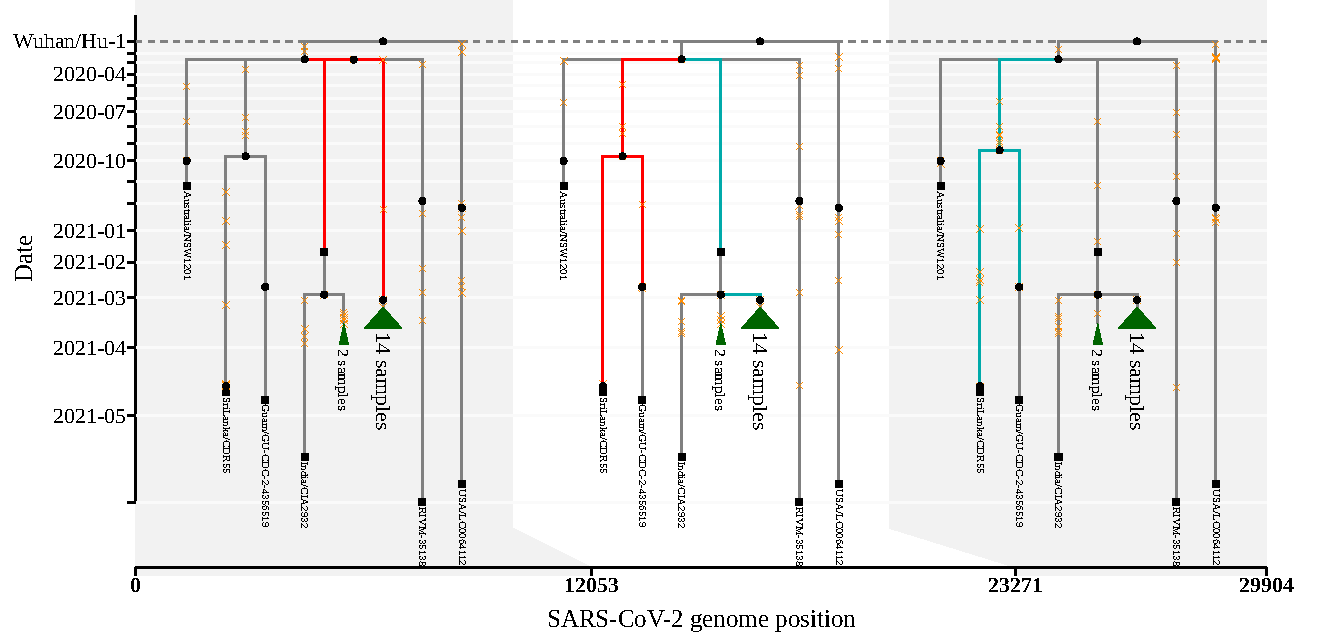
\includegraphics[width=\textwidth]{Covid_recombination}

\end{posterbox}
%%%%%%%%%%%%%%%%%%%%%%%%%%%%%%%%%%%%%%%%%%%%%%%%%%%%%%%%%%%%%%%%%%%%%%%%%%%%%%



%%%%%%%%%%%%%%%%%%%%%%%%%%%%%%%%%%%%%%%%%%%%%%%%%%%%%%%%%%%%%%%%%%%%%%%%%%%%%%
\begin{posterbox}[name=stats,column=3,row=0,span=1]{Statistics}
%%%%%%%%%%%%%%%%%%%%%%%%%%%%%%%%%%%%%%%%%%%%%%%%%%%%%%%%%%%%%%%%%%%%%%%%%%%%%%

\tskit{} lets you perform efficient calculations of statistics along the genome, often many times quicker than other software! You may be interested in calculating...

\begin{itemize} \compresslist
    \item statistics derived from the allele frequency spectrum like nucleotide diversity, Tajima's D, f2...
    \item IBD-based quantities
    \item tree-based statistics like genealogical nearest neighbours and tree balance metrics...
\end{itemize}

Let's look at \tskit{}'s new tree balance statistics as an example. A balanced
    (binary) tree is perfectly symmetric in some way: each node has an equally
    sized subtree descending from its left- and right- branches, where 'size'
    is determined by some metric involving the tree's nodes and edges. \tskit
    now contains several different metrics to calculate how unbalanced each
    tree is:

\begin{minted}{python}
imb = pd.DataFrame({
    "genomic position" : [t.interval[0] for t in ts.trees()],
    "b1" : [t.b1_index() for t in ts.trees()],
    "b2" : [t.b2_index() for t in ts.trees()],
    "colless" : [t.colless_index() for t in ts.trees()],
    "sackin" : [t.sackin_index() for t in ts.trees()]
}).set_index("genomic position")

imb = ((imb - imb.mean()) / imb.std())
imb.plot(figsize=(16, 4), alpha=0.7)
\end{minted}
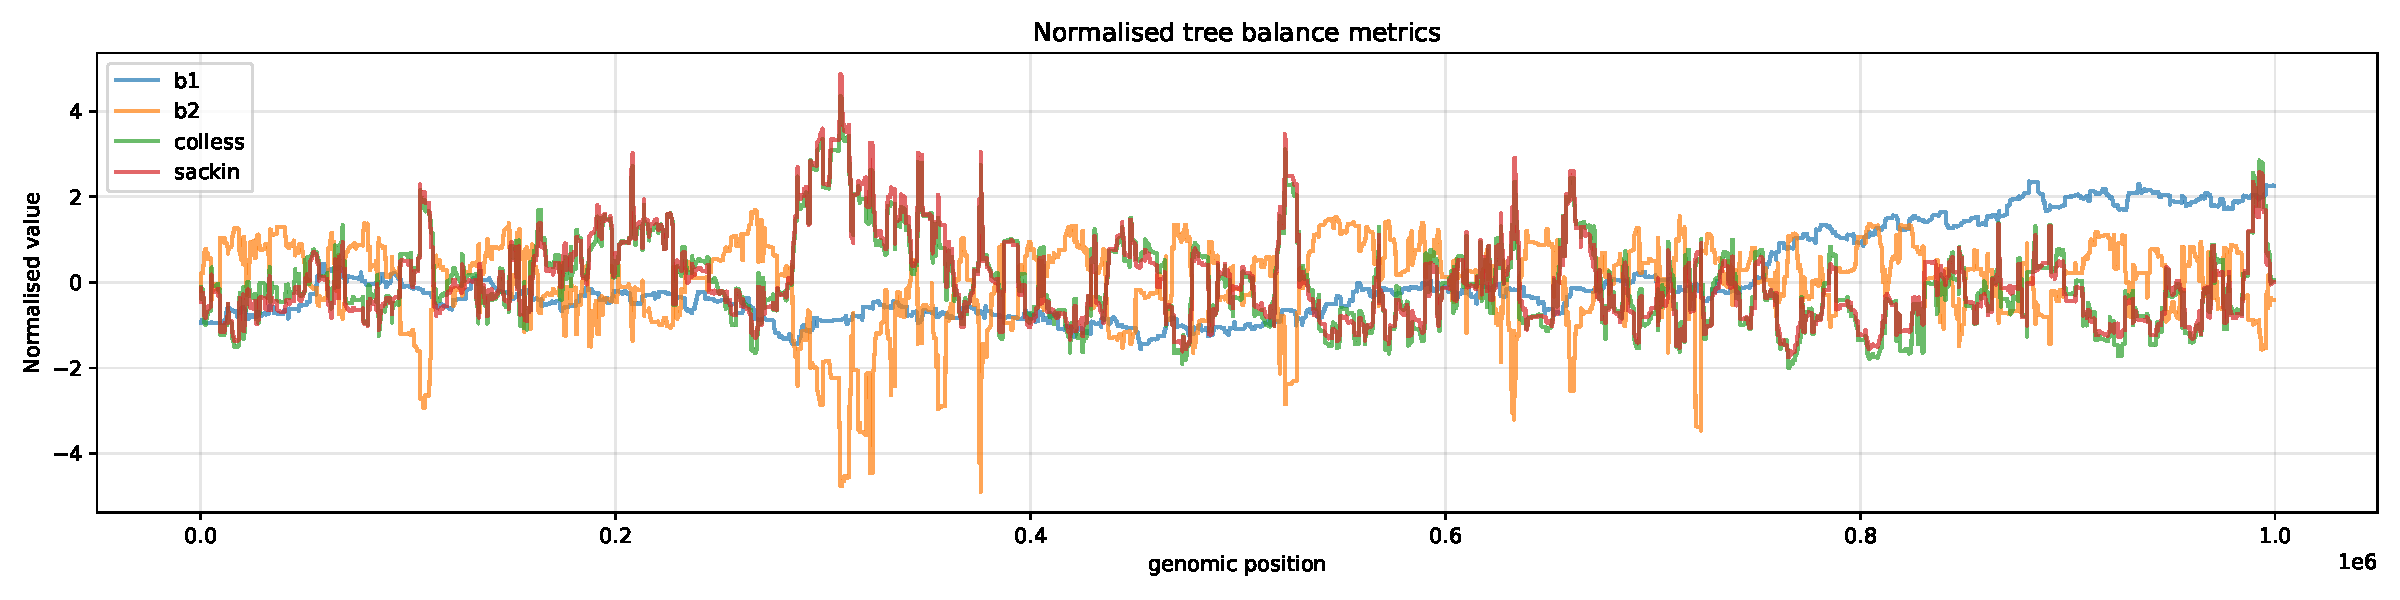
\includegraphics[width=\textwidth]{tree_balance}

\end{posterbox}
%%%%%%%%%%%%%%%%%%%%%%%%%%%%%%%%%%%%%%%%%%%%%%%%%%%%%%%%%%%%%%%%%%%%%%%%%%%%%%


%%%%%%%%%%%%%%%%%%%%%%%%%%%%%%%%%%%%%%%%%%%%%%%%%%%%%%%%%%%%%%%%%%%%%%%%%%%%%%
\begin{posterbox}[name=operations,column=3,below=stats,span=1]{Notable new features}
%%%%%%%%%%%%%%%%%%%%%%%%%%%%%%%%%%%%%%%%%%%%%%%%%%%%%%%%%%%%%%%%%%%%%%%%%%%%%%

\tskit{}'s contributors are diverse and prolific! We are actively working on new features, bug fixes, and improvements to the usability of existing features. Here's a shortlist of some recent additions:

\paragraph{Reference sequences}
By default, the sites in a tree sequence only define the nucleotide types at
    the genomic positions where polymorphism is observed. The nucleotides at
    remaining positions can now be filled using the
    `TreeSequence.reference\_sequence` , and individual sample alignments can
    be obtained with the new `TreeSequence.alignments()` iterator.

\paragraph{Structural operations}
We've expanded the set of utility functions for large edits on tree sequences.
    For instance, the `TreeSequence.decapitate` method removes all parts of a
    tree sequence that are older than some user-specified time.

\paragraph{Efficient array access }
The relationships between nodes in each tree can now be extracted as `numpy`
    arrays. When used in conjunction with `numba`, it is possible to perform
    Python-based calculations on the trees that run as speedily as
    machine-level code. Consider these calculations of total branch length on
    trees of different sizes:

\begin{minted}{python}
@numba.njit
def _total_branch_length(preorder, parent, node_time):
     tbl = 0
     for u in preorder:
          if parent[u] != -1:
               tbl += node_time[parent[u]] - node_time[u]
     return tbl

def get_total_branch_length(tree):
     return _total_branch_length( tree.preorder(), tree.parent_array,
                tree.tree_sequence.nodes_time)
\end{minted}
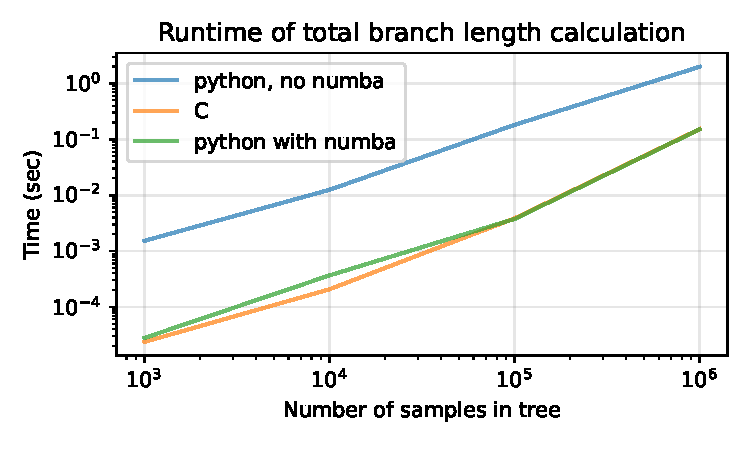
\includegraphics[width=0.5\textwidth]{numba_runtime}

\end{posterbox}
%%%%%%%%%%%%%%%%%%%%%%%%%%%%%%%%%%%%%%%%%%%%%%%%%%%%%%%%%%%%%%%%%%%%%%%%%%%%%%



%%%%%%%%%%%%%%%%%%%%%%%%%%%%%%%%%%%%%%%%%%%%%%%%%%%%%%%%%%%%%%%%%%%%%%%%%%%%%%
\begin{posterbox}[name=refs,column=1,above=bottom]{Contributors}
%%%%%%%%%%%%%%%%%%%%%%%%%%%%%%%%%%%%%%%%%%%%%%%%%%%%%%%%%%%%%%%%%%%%%%%%%%%%%%

    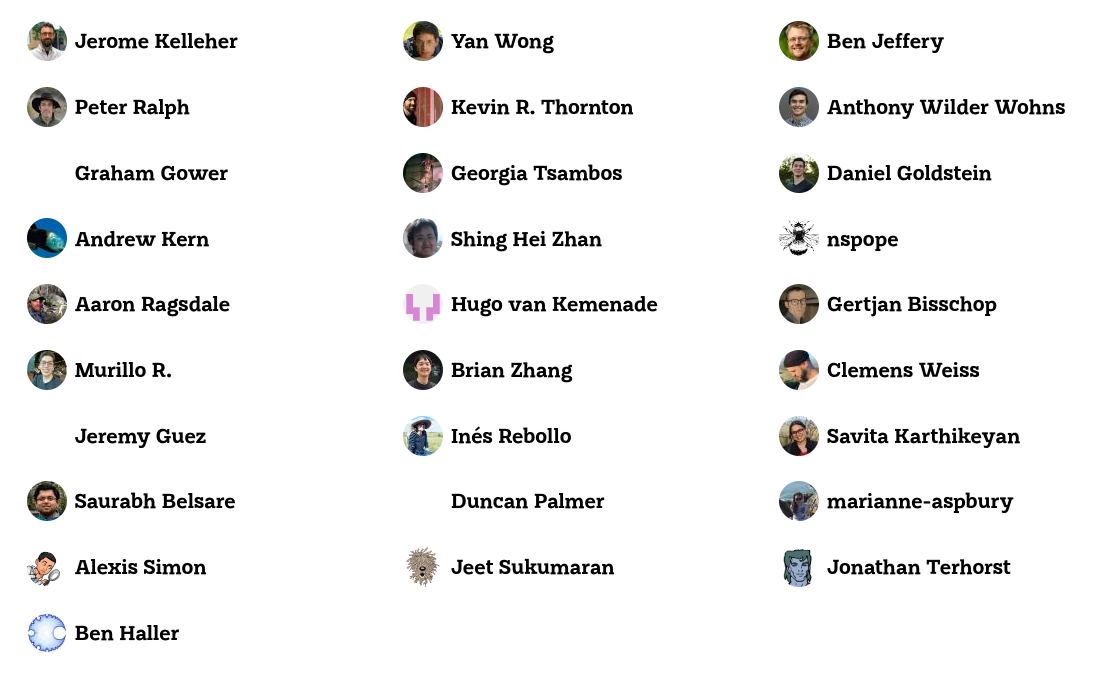
\includegraphics[width=\textwidth]{tskit-contributors}

  % % \scriptsize
  % \renewcommand{\section}[2]{\vskip 0.0em}
  % \bibliographystyle{abbrvnat}
  % \setlength{\bibsep}{0.0pt}

  % \bibliography{refs}
\end{posterbox}
%%%%%%%%%%%%%%%%%%%%%%%%%%%%%%%%%%%%%%%%%%%%%%%%%%%%%%%%%%%%%%%%%%%%%%%%%%%%%%


\end{poster}%
\end{document}
